
\subsection{The Low-$\nu$ Sky: Emission Mechanisms}
\pg
This section aims to bring a brief introduction to the emission mechanisms which dominate at low frequencies, and thus determine the physics accessible to extragalactic astronomers working in this band. Specifically, it will briefly describe
%thermal radiation detected at low frequencies (associated with dust \& protoplanetary disks, and therefore a tracer of star formation) along with 
free-free radiation (which is emitted from ionised plasma outflows, and thus a tracer of various physical objects e.g. young stellar objects - cf. \citet{2017ApJ...834..206C} and references therein - and starburst regions - cf. \citet{2015A&A...574A.114V}) and synchrotron radiation, which is a tracer of more violent and energetic processes (and thus associated with supernova remnants, AGN, or radio halos - cf. \citet{2010A&A...509A..68C}).

\pg
Of course, each individual galaxy will have differing contributions from different mechanisms - in practice, when studying galactic populations, the overall flux at a given frequency will simply be summed up for each galaxy and become one point in a Spectral Energy Distribution, or SED. However, when studying individual objects, it can be critical to understand which emission mechanism dominates at what frequencies. %: it will be very difficult to find traces of star formation in the emission from a galaxy dominated by an AGN, for example. Along with a brief introduction of the main emission mechanisms, then, we will give the characteristic spectrum of each, to show how different types of emission can be differentiated in practice.
For example, the radio and far-infrared spectrum for nearby M82 are shown in Fig. \ref{plot.m82.spectrum}\footnote{Figure and work taken from the NRAO website. For further information, \href{https://www.cv.nrao.edu/course/astr534/FreeFreeEmission.html}{see here}}.
\begin{figure*}[!h]
\centering
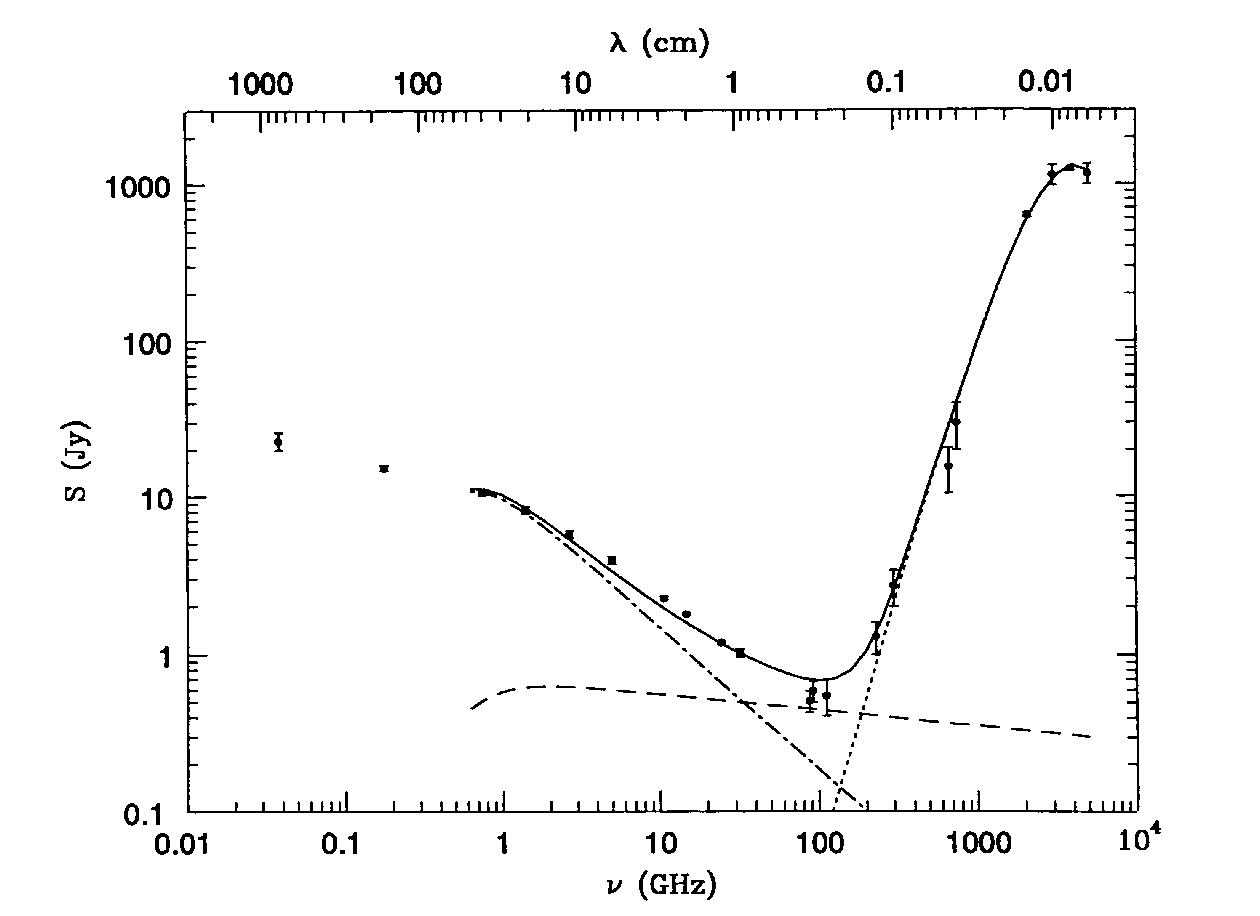
\includegraphics[width=\textwidth]{images/M82Spectrum.png}
\caption{\label{plot.m82.spectrum} Radio and far-infrared spectrum for galaxy M82, as estimated \href{https://www.cv.nrao.edu/course/astr534/FreeFreeEmission.html}{by the NRAO online course}. The flat curve corresponds to free-free emission, while synchrotron radiation and thermal dust emission dominate at low and high frequencies respectively.}
\end{figure*}


\subsubsection{Synchrotron Radiation}

\pg
Synchrotron radiation is the dominant mode of emission for extragalactic sources at low wavelengths. As such, it will be covered in greater detail that the other mechanisms above, which are important in other bands (and therefore relevant for multi-spectral analysis) but much less relevant to LOFAR observations. This section draws heavily from Garret Cotter's \href{http://www-astro.physics.ox.ac.uk/~garret/teaching/}{high-energy astrophysics lectures}, as well as Alan Loh's \href{http://theses.md.univ-paris-diderot.fr/LOH_Alan_2_va_20160930.pdf}{doctoral thesis} and \href{https://www.cv.nrao.edu/course/astr534/SelfAbsorption.html}{the NRAO online course}.

\pg
Synchrotron radiation (or "magnetobremsstrahlung") occurs when the trajectory of a relativistic charged particle is deflected by a magnetic field. As the German name suggests, it is the magnetic equivalent of free-free radiation. It is the tracer of very energetic processes, such as the interaction between AGN jets and the intergalactic medium. In the low-energy regime, it is also known as cyclotron radiation, after the device in which it was first measured in a laboratory. %, and in non-relativistic regimes, it is known as gyro radiation. 

\pg
The synchrotron power spectrum of a population of electrons with exactly the same energy is a function of its Lorentz factor and its emission angle\footnote{The emission angle is the angle between the electron's velocity and its radial velocity.} \citepads{1994hea2.book.....L}. The typical radiation spectrum for a single electron is shown in \cref{fig.synchrotron.1electrion} as a function of the critical frequency, which is itself a function of the emission angle and the synchrotron frequency\footnote{Which is itself a function of the Lorentz factor and the magnetic field strength - $\nu_\mathrm{sync}=\frac{\gamma^2 e B}{2\pi m_e c}$ .}: $\nu_c=3/2\nu_\mathrm{sync}\sin(\theta)$.
\begin{figure}[!h]
\centering
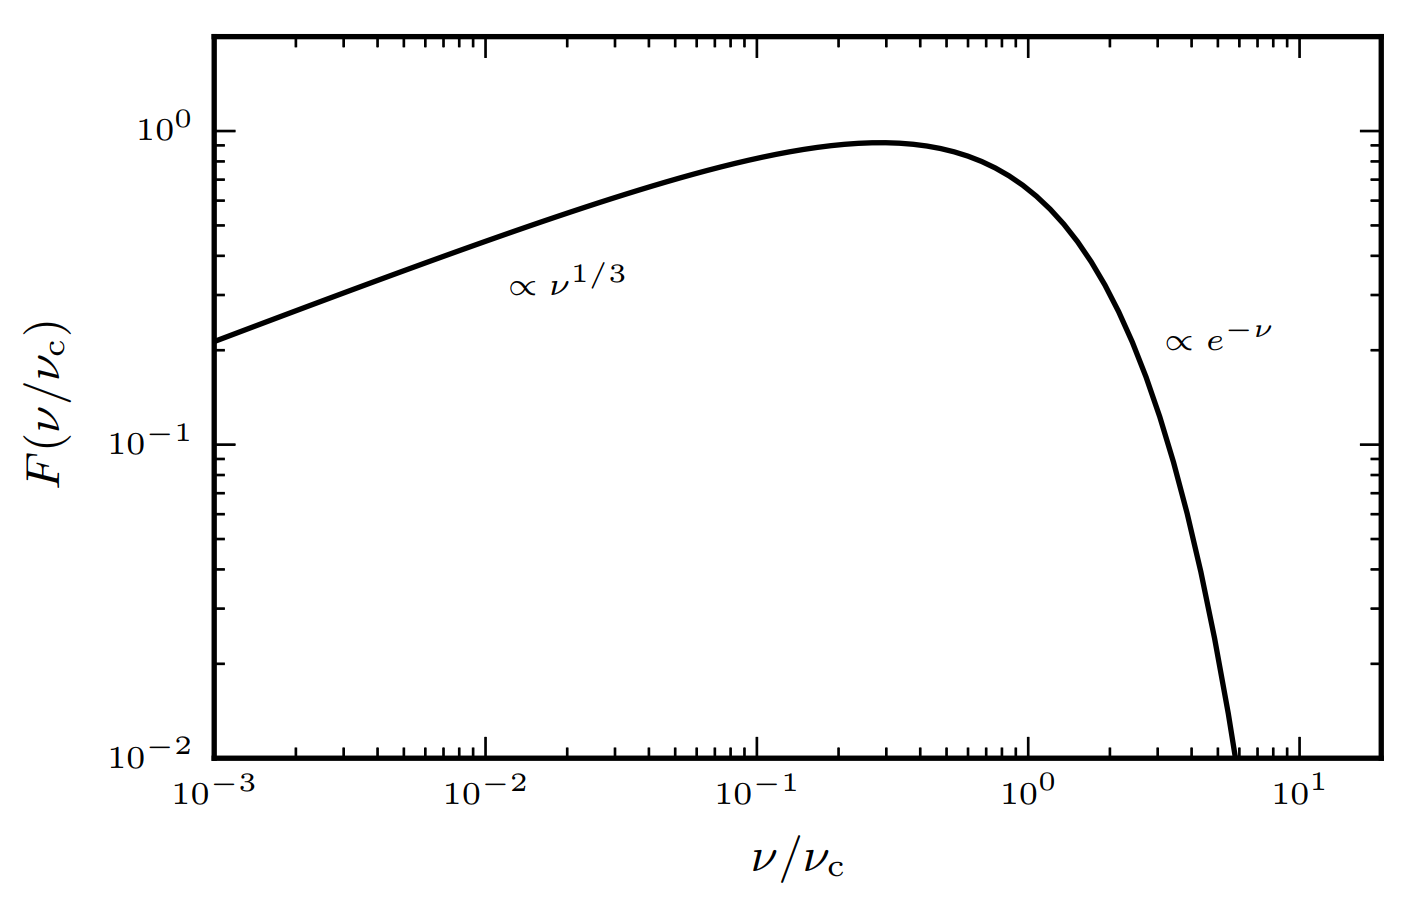
\includegraphics[width=0.9\textwidth]{images/Synchrotron-single-electron.png}
\caption{\label{fig.synchrotron.1electrion} Characteristic spectrum of synchrotron emission for a population of single-energy electrons. Arbitrary unit scale. Source: NRAO online course.}
\end{figure}

\pg
Of course, in reality, we know that electron populations in astrophysical sources do not all share exactly the same energy when emitting. The effect of the electron energy distribution must therefore be taken into account. Because the population in question is energised through non-thermal processes, its energy distribution is not Maxwellian, and is generally written as a power law: $S_\nu \propto \nu^{\alpha}$, where $\alpha$ is the object's spectral index. %If the dominant mechanism for charged particle acceleration is Fermi acceleration (see \citetads{1978MNRAS.182..147B} and companion papers, \citetads{2007Ap&SS.309..119R}), aggregate spectrum can be described as a power law in Lorentz factor:
%\begin{align}
%P_\mathrm{sync} (\nu,\theta) &= \kappa B^{.5(p+1)} \nu^{-.5(p-1)}
%\end{align} 
The question now becomes: what $\alpha$ is appropriate for what kind of object? Does every source have the same $\alpha$ at all frequencies? Do all synchrotron sources have the same spectral index at a given frequency, and if not, what does this tell us?

\pg
To answer these questions, we must recall that so far, we have assumed that every photon emitted through synchrotron radiation reaches us. This is not necessarily the case in practice: it is possible for a given photon to be scattered (i.e. absorbed \& re-emitted) by surrounding synchrotron electrons. The likelihood of this occurring at a given frequency is a function of the absorption cross-section, and is a complex quantity to calculate (see \citetads{1994hea2.book.....L} pp258-260). Suffice to say that at longer wavelengths (lower frequencies) absorption is more effective, and at shorter wavelengths (higher frequencies) the underlying electron energy power-law  distribution can be seen. An example is shown in \cref{fig.synchrotron}, taken from \citetads{2007A&A...471.1105T,}.

\begin{figure}[!h]
\centering
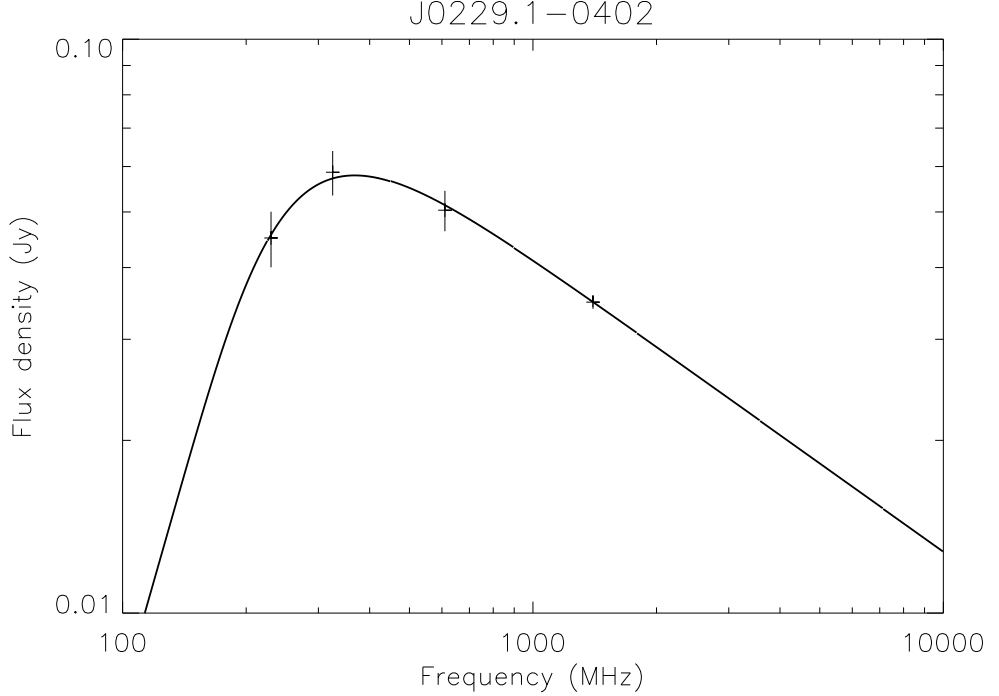
\includegraphics[width=0.8\textwidth]{images/synchrotron-spectrum.png}
\caption{\label{fig.synchrotron} Power spectrum for J0229.1-0402.}
\end{figure}

\pg
In the optically-thick regime, we know that the most efficient radiation mechanism is simple black-body radiation, and so the power spectrum at a given frequency can be defined in terms of an ``electron temperature". In the Rayleigh-Jeans approxmation (valid as we are explicitly in the low-frequency regime), this gives $S_\nu \propto \nu{5/2}$, or $\alpha=5/2$. 
In the optically-thin regime, meanwhile, we recover a mixture of the underlying power-law distribution ($S_\nu \propto e^{-\nu}$) and black-body radiation (which has a frequency-dependent $\alpha$). Empirically, we generally observe $\alpha \sim 0.7$.


%\subsection{Thermal Radiation}
%\pg
%Also known as black-body radiation, its spectral intensity is given by Planck's law, given in Eq. \ref{eq.planck}.
%\begin{equation}\label{eq.planck}
%%B_\lambda (\lambda,T) = \frac{2hc^2}{\lambda^5}\left(e^{\frac{hc}{\lambda k_BT}}-1\right)^{-1}
%B_\nu(\nu,T) = \frac{2h\nu^3}{c^2}\left(e^\frac{h\nu}{k_BT}-1\right)^{-1}
%\end{equation}
%where $B_\lambda$ is the flux density at frequency $\nu$ for a source with temperature $T$, and $k_B=1.381 \left[J/K\right]$ is the Boltzmann constant. Near protostellar disks, synchrotron emission is absorbed by the ambient interstellar medium, heating it up to an average of $\sim 10^4$ (see \citetads{2009ApJS..181..255A}, \citetads{1978ppim.book.....S} and references therein). Assuming that the interstellar medium is optically thick at all frequencies, this gives the following spectral curve:
%
%\begin{figure*}[!h]
%\centering
%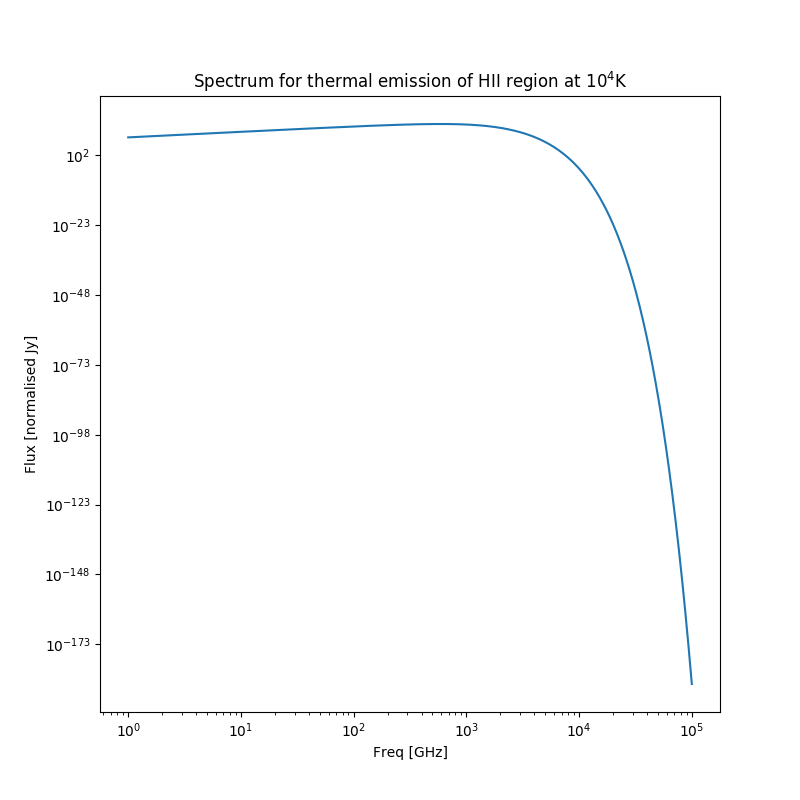
\includegraphics[width=0.8\textwidth]{images/ThermalEmission.png}
%\caption{\label{plot.thermal}Log-Log plot of blackbody radiation emitted by a particle at $10^4$ Kelvin. Note that the y-axis is arbitrary, since it will in practice be modulated by density, radiation efficiency, resolution etc.}
%\end{figure*}
%\pg
%This is the dominant mode of emission for distant galaxies in the infrared band, but is not expected to contribute in the LOFAR regime for extragalactic sources. It ought to be detected for nearby resolved galaxies, however.

\subsubsection{Free-Free Radiation}
\pg
Free-free or ``bremsstrahlung" (``braking") radiation occurs when the trajectory of a charged particle is deflected by an electric field. This non-thermal emission mechanism is the dominant mechanism in HII regions (which contain ionised hydrogen), where star formation has previously taken place. It is called free-free emission because it is produced by free electrons deviating off ionised hydrogen without being captured. When the underlying electron distribution is Maxwellian, it is referred to as thermal Bremsstrahlung.% as shown in Fig. \ref{plot.freefree}
%\begin{figure*}[!h]
%\centering
%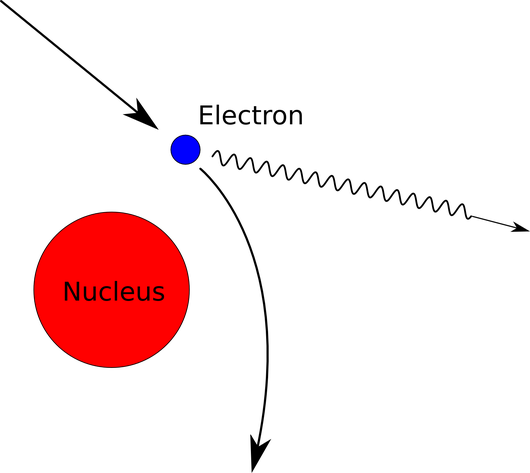
\includegraphics[width=0.3\textwidth]{images/bremsstrahlung.png}
%\caption{\label{plot.freefree} Schematic showing the physical process leading to free-free emission. As we can see, the electron is scattered, but not captured. Source: \url{https://thephysicsbehind.com/2015/04/16/x-ray-tubes/}}
%\end{figure*}

\pg
This emission's spectrum is heavily dependent on a number of factors: including frequency, temperature, and critically, free-free opacity $\tau_\nu$, itself a function of electron density. It is characterised by a knee in its spectrum, occurring where $\tau_\nu\sim 1$. This knee delineates two regions with different spectral indices; $\alpha \sim -0.1$ at higher frequencies, and $\alpha \leq 2$ at lower frequencies. This gives a characteristic shape, shown in Fig. \ref{plot.freefree.spectrum}.
\begin{figure*}[!h]
\centering
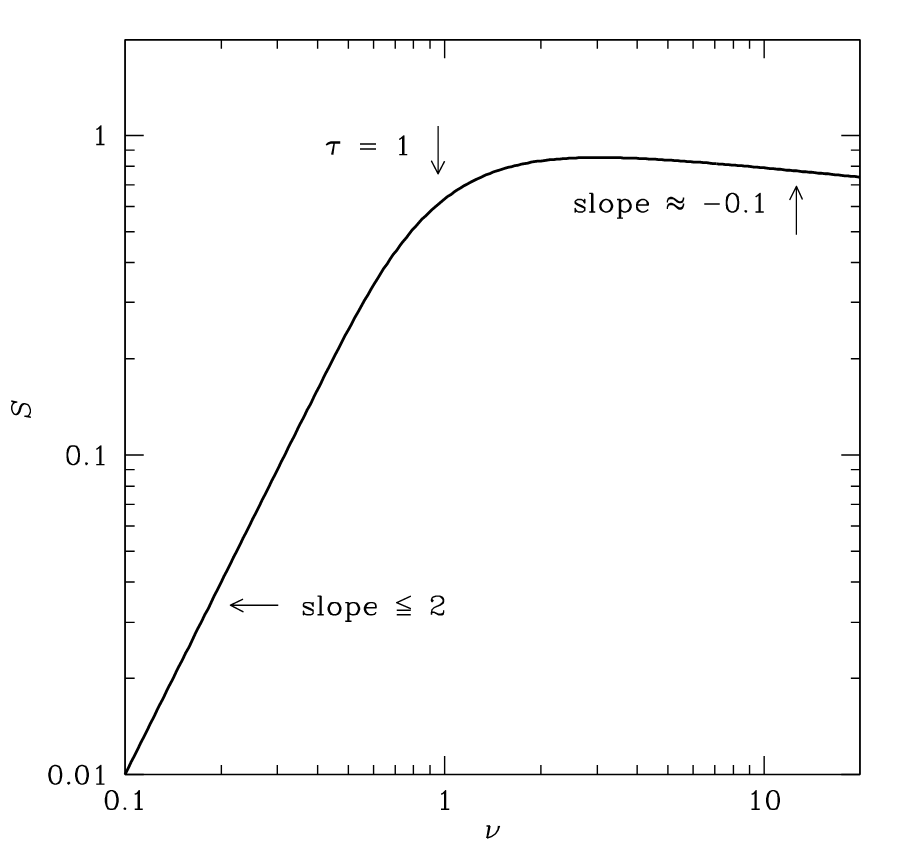
\includegraphics[width=0.8\textwidth]{images/freefree.png}
\caption{\label{plot.freefree.spectrum} Characteristic spectrum of free-free radiation. Arbitrary unit scale. Source: NRAO online course.}
\end{figure*}

\pg
As we can see, this spectrum falls off sharply with frequency. As such, while it is expected to dominate over thermal emission in the absence of synchrotron radiation, it is synchrotron emission that is expected to dominate overall - if present - in the LOFAR band. Free-free emission acts as a tracer for star formation and other "gentler" physical processes detected at low radio frequencies.
